\documentclass[11pt,a4paper]{article}
\usepackage[margin=2.3cm]{geometry}
\usepackage{lmodern}
\usepackage[T1]{fontenc}
\usepackage{amsmath,amssymb}
\usepackage{booktabs,tabularx,array}
\usepackage{graphicx}
\usepackage{xcolor}
\usepackage{enumitem}
\usepackage{float}
\usepackage{caption}
\usepackage[hidelinks]{hyperref}
\definecolor{muted}{HTML}{52514e}
\setlist{nosep,leftmargin=1.4em}
\captionsetup{font=small,labelfont=bf}
\newcommand{\note}[1]{\par\smallskip{\footnotesize\color{muted}#1}}

\title{\textbf{Mis-selling, Lapse and Planner Settlement}\\[4pt]
\large A Company-Level Panel Study of Korean Insurers, 2021--2025}
\author{Actuarial study note}
\date{5 October 2026}

\begin{document}
\maketitle

\begin{abstract}
\noindent Using company-level public disclosures from the Financial Supervisory Service (FSS) and the General
Insurance Association of Korea (KNIA), we build an annual panel of 14 non-life insurers (2021--2025) linking
the mis-selling rate, 13th- and 25th-month lapse rates and the one-year settlement (retention) rate of newly
registered exclusive planners, plus a 23-insurer life panel without mis-selling data. We estimate pooled, random-effects,
firm fixed-effects and two-way fixed-effects models with firm-clustered and wild-cluster-bootstrap inference.
Three findings stand out. (1) Mis-selling and lapse are strongly correlated \emph{across} insurers
(between-firm $r=0.84$), but the association disappears \emph{within} insurers over time (within $r=0.15$,
two-way FE coefficient insignificant); the cross-sectional link reflects business model, with
telemarketing- and direct-led insurers high on both. (2) Planner settlement is the robust predictor: within a
non-life insurer, a 10 percentage-point (pp) higher settlement rate is associated with a 0.95\,pp lower
13th-month lapse rate (two-way FE, $p=0.014$; wild-bootstrap $p=0.047$), and the effect is larger excluding
TM/direct insurers. (3) Settlement is unrelated to mis-selling within firms, and in the life sector the
settlement--lapse link is weaker and not robust to year effects.
\end{abstract}

\tableofcontents

%====================================================================
\section{Introduction}
%====================================================================
The commission reform analysed in our companion note (the 1200\% rule and installment payments) rests on a
behavioural premise: sales practices driven by upfront pay produce poor-quality business that lapses early,
and unstable sales forces leave ``orphan'' policies that nobody services. Korean regulators publish three
company-level indicators that speak directly to that premise:
\begin{itemize}
  \item the \textbf{mis-selling rate} (\emph{bulwanjeon panmae biyul}): quality-guarantee cancellations,
        complaint cancellations and voided contracts as a share of new contracts;
  \item the \textbf{13th- and 25th-month persistency} of premium (we use lapse $=100-$ persistency);
  \item the \textbf{planner settlement rate}: the share of newly registered exclusive planners still active one year later.
\end{itemize}
We ask three questions:
\begin{enumerate}
  \item[\textbf{Q1}] Do insurers with more mis-selling have higher lapse rates---and does a given insurer's lapse rise when its mis-selling rises?
  \item[\textbf{Q2}] Is a more stable sales force (higher settlement) associated with lower lapse?
  \item[\textbf{Q3}] Is a more stable sales force associated with less mis-selling?
\end{enumerate}
The panel structure lets us separate \emph{between-firm} differences (business model, channel mix, product mix),
which are permanent, from \emph{within-firm} changes over time, which are closer to the causal question regulators care about.

%====================================================================
\section{Data}
%====================================================================
\subsection{Sources}
\begin{itemize}
  \item \textbf{FSS insurance company disclosure, ``Contract management''} (\url{https://www.fss.or.kr/fss/bbs/B0000117/list.do?menuNo=200414}).
        For every life and non-life insurer: settlement rate of exclusive planners and 13th/25th-month persistency.
        We use the five calendar-year windows 2021, 2022, 2023, 2024 and 2025. Overlapping July--June windows
        are excluded to avoid double counting.
  \item \textbf{KNIA consumer portal disclosures} (\url{https://consumer.knia.or.kr/disclosure/item/07.do} and item 04).
        Item 04: mis-selling rate by channel and company, by half-year, 2020H1--2026H1. Item 07 (the page
        supplied): long-term claim denial rate and post-claim cancellation rate with underlying counts, by half-year.
        KNIA covers non-life insurers only; the life association publishes the life equivalent separately, so
        the mis-selling analysis is restricted to non-life.
\end{itemize}
All pages were downloaded on 5 October 2026; the raw HTML is archived with the code.

\subsection{Construction}
Company names were harmonised across renamings and mergers (e.g.\ MG $\to$ Yebyeol, Shinhan Life $=$ Shinhan +
Orange Life from July 2021, KB Life $=$ KB Life + Prudential from 2023, DGB $\to$ iM Life). The KNIA annual
mis-selling rate is the mean of the two half-yearly all-channel rates; annual claim denial and post-claim
cancellation rates are recomputed from summed counts. Reported values of exactly 0.0 for settlement or persistency
(companies with no newly registered exclusive planners in the window) are treated as missing. Meritz is missing
from KNIA's 2024 mis-selling tables.

\paragraph{Timing.} Persistency published for year $t$ is measured on contracts written 12 months (13th month)
or 24 months (25th month) earlier. We therefore pair 13th-month lapse in $t$ with mis-selling in $t-1$, and
25th-month lapse in $t$ with mis-selling in $t-2$ and settlement in $t-1$. This also reduces simultaneity.

\paragraph{Sample.} The non-life analysis sample has 14 insurers (11 face-to-face-led; AIG, ACE/Lina and AXA
are telemarketing/direct-led). Three digital or sparsely reported insurers (Shinhan EZ, Kakao Pay, Cardif)
are excluded. ACE/Lina reports no settlement rate, so regressions that include settlement have 13 firms.

\begin{table}[H]\centering\small
\caption{Non-life panel: descriptive statistics, 2021--2025. ``Between'' is the SD of firm means; ``within'' the SD of deviations from firm means.}
\begin{tabular}{lrrrrrr}
\toprule
Variable & $N$ & Firms & Mean & SD & SD between & SD within \\
\midrule
13th-month lapse (\%) & 70 & 14 & 17.49 & 8.04 & 7.89 & 2.46 \\
25th-month lapse (\%) & 70 & 14 & 31.57 & 8.64 & 8.07 & 3.63 \\
Planner settlement (\%) & 64 & 13 & 50.77 & 17.28 & 15.44 & 9.57 \\
Mis-selling rate (bp) & 69 & 14 & 3.38 & 4.60 & 3.95 & 2.50 \\
Claim denial rate (\%) & 70 & 14 & 1.53 & 0.50 & 0.40 & 0.31 \\
Post-claim cancellation (\%) & 70 & 14 & 0.26 & 0.32 & 0.31 & 0.10 \\
\bottomrule
\end{tabular}
\end{table}
\begin{table}[H]\centering\small
\caption{Life panel: descriptive statistics, 2021--2025.}
\begin{tabular}{lrrrrrr}
\toprule
Variable & $N$ & Firms & Mean & SD & SD between & SD within \\
\midrule
13th-month lapse (\%) & 111 & 23 & 15.52 & 5.47 & 2.85 & 4.67 \\
25th-month lapse (\%) & 111 & 23 & 32.63 & 9.84 & 5.06 & 8.50 \\
Planner settlement (\%) & 77 & 20 & 34.95 & 15.71 & 14.27 & 8.44 \\
\bottomrule
\end{tabular}
\end{table}
\noindent Two features of the data shape everything that follows. First, most variation is \emph{between} firms:
the between-firm SD of 13th-month lapse (7.9\,pp) is three times the within-firm SD (2.5\,pp). Second, the
mis-selling rate is tiny and coarsely reported. KNIA publishes it to two decimals of a percent, so face-to-face
insurers mostly show 1--3 basis points (bp), while AIG and ACE/Lina show 5--25\,bp (Figure~\ref{fig:trend}).
Mis-selling also fell steeply industry-wide after 2020.

\begin{figure}[H]\centering
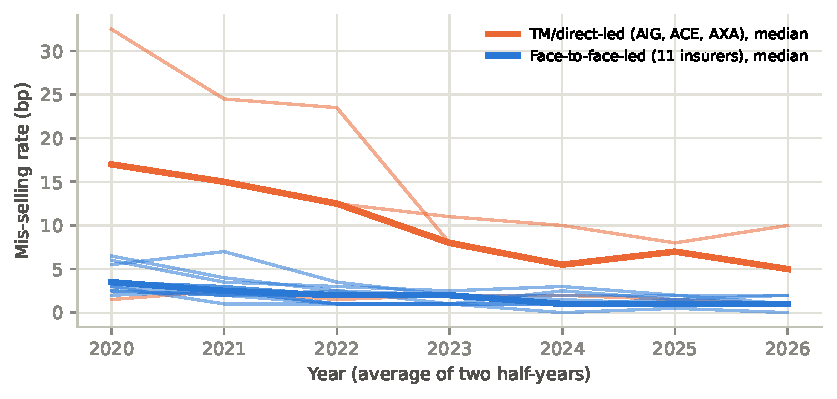
\includegraphics[width=0.92\linewidth]{fig/ms_trend.pdf}
\caption{Non-life mis-selling rate by insurer (thin lines) and group medians (thick). The level gap is between business models; the decline is common to all.\note{Source: KNIA consumer portal, item 04; annual mean of half-year all-channel rates.}}\label{fig:trend}
\end{figure}

%====================================================================
\section{Method}
%====================================================================
For firm $i$ in year $t$ we estimate
\begin{equation}
  y_{it} = \alpha_i + \lambda_t + \beta\,\mathrm{MS}_{i,t-\ell} + \gamma\,\mathrm{Settle}_{i,t-m} + \varepsilon_{it},
\end{equation}
with $y$ the 13th- or 25th-month lapse rate. Five estimators are reported side by side:
\begin{itemize}
  \item \textbf{Pooled OLS}: no $\alpha_i$, no $\lambda_t$. Mixes between- and within-firm variation.
  \item \textbf{Year FE}: adds $\lambda_t$ only. Comparisons are among insurers in the same year.
  \item \textbf{Random effects (RE)}: treats $\alpha_i$ as random and uncorrelated with the regressors.
  \item \textbf{Firm FE}: absorbs all time-invariant firm characteristics (channel mix, product mix, brand).
  \item \textbf{Two-way FE (TWFE)}: firm and year effects. Identification comes only from a firm's change
        relative to the industry's change in the same year. This is our preferred specification.
\end{itemize}
Standard errors are clustered by firm. Because 13 clusters is few, key coefficients are also tested with a
wild cluster restricted bootstrap (Webb six-point weights, 9{,}999 draws, null imposed). A Hausman test
compares FE and RE. We complement the regressions with a \textbf{correlation decomposition}: the pooled
correlation, the between correlation of firm means, and the within correlation after removing firm and year means.

%====================================================================
\section{Results}
%====================================================================
\subsection{Correlation decomposition}
\begin{table}[H]\centering\small
\caption{Pooled, between-firm and within-firm (firm- and year-demeaned) correlations. $^{*}$, $^{**}$, $^{***}$: $p<0.10, 0.05, 0.01$.}
\begin{tabular}{llrrrr}
\toprule
Sample & Pair ($x$, $y$) & $N$ (firms) & Pooled $r$ & Between $r$ & Within $r$ \\
\midrule
Non-life & Mis-selling$_{t-1}$, Lapse13$_t$ & 69 (14) & $0.67^{***}$ & $0.84^{***}$ & $0.15$ \\
Non-life & Mis-selling$_{t-2}$, Lapse25$_t$ & 56 (14) & $0.65^{***}$ & $0.83^{***}$ & $0.14$ \\
Non-life & Settlement$_t$, Lapse13$_t$ & 64 (13) & $-0.67^{***}$ & $-0.78^{***}$ & $-0.42^{***}$ \\
Non-life & Settlement$_{t-1}$, Lapse25$_t$ & 51 (13) & $-0.58^{***}$ & $-0.66^{**}$ & $-0.41^{***}$ \\
Non-life & Settlement$_t$, Mis-selling$_t$ & 63 (13) & $-0.26^{**}$ & $-0.34$ & $0.03$ \\
Non-life & Claim denial$_t$, Lapse13$_t$ & 70 (14) & $0.27^{**}$ & $0.44$ & $-0.25^{**}$ \\
Life & Settlement$_t$, Lapse13$_t$ & 77 (20) & $-0.30^{***}$ & $-0.26$ & $-0.17$ \\
Life & Settlement$_{t-1}$, Lapse25$_t$ & 62 (19) & $-0.09$ & $0.02$ & $-0.13$ \\
\bottomrule
\end{tabular}
\note{Within-correlation $p$-values do not adjust for degrees of freedom absorbed by demeaning and are indicative only; regression inference follows below.}
\end{table}
The decomposition already answers much of Q1--Q3 (Figure~\ref{fig:bw}):
\begin{itemize}
  \item \textbf{Mis-selling--lapse}: very strong between firms ($r=0.84$) but weak and insignificant within firms ($r=0.15$).
  \item \textbf{Settlement--lapse}: negative at every level, including within firms ($r=-0.42$ for 13th month,
        $-0.41$ for 25th month, both $p<0.01$).
  \item \textbf{Settlement--mis-selling}: weakly negative pooled, zero within ($r=0.03$).
\end{itemize}

\begin{figure}[H]\centering
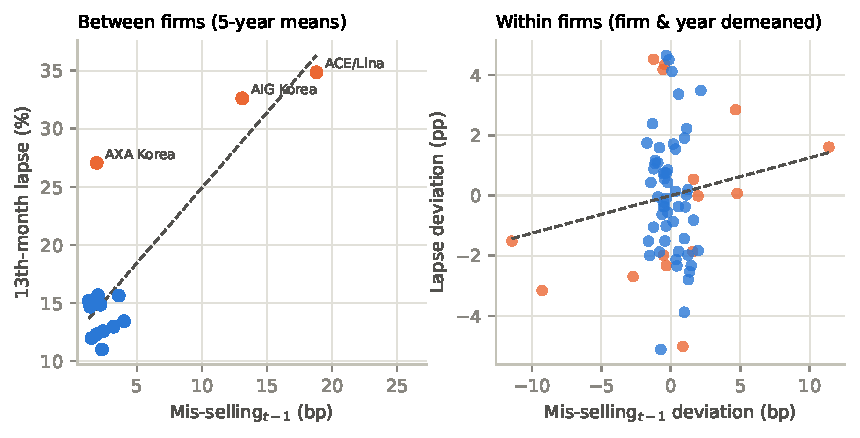
\includegraphics[width=0.95\linewidth]{fig/between_within_ms.pdf}
\caption{Mis-selling$_{t-1}$ vs.\ 13th-month lapse. Left: firm means; orange points are TM/direct-led insurers. Right: firm- and year-demeaned observations (bivariate fit). The between-firm slope is driven by business model; within firms the relationship is flat.}\label{fig:bw}
\end{figure}

\subsection{Q1 and Q2: what predicts lapse?}
\begin{table}[H]\centering\small
\caption{13th-month lapse$_t$ (\%), non-life. Firm-clustered SE in parentheses.}
\begin{tabular}{lccccc}
\toprule
 & Pooled OLS & Year FE & Random eff. & Firm FE & Two-way FE \\
\midrule
Mis-selling$_{t-1}$ (bp) & $0.901^{***}$ & $1.084^{***}$ & $0.231$ & $-0.724^{**}$ & $-0.698$ \\
 & $(0.178)$ & $(0.159)$ & $(0.205)$ & $(0.338)$ & $(0.560)$ \\
Settlement$_t$ (\%) & $-0.219^{***}$ & $-0.202^{***}$ & $-0.163^{***}$ & $-0.083^{**}$ & $-0.095^{**}$ \\
 & $(0.047)$ & $(0.050)$ & $(0.024)$ & $(0.034)$ & $(0.037)$ \\
\midrule
$N$ (firms) & 63 (13) & 63 (13) & 63 (13) & 63 (13) & 63 (13) \\
$R^2$ (within for FE) & 0.64 & 0.71 & 0.31 & 0.29 & 0.23 \\
Hausman FE vs RE & \multicolumn{5}{c}{$\chi^2(2)=80.15$, $p=0.000$} \\
\bottomrule
\end{tabular}
\end{table}
\begin{table}[H]\centering\small
\caption{25th-month lapse$_t$ (\%), non-life.}
\begin{tabular}{lccccc}
\toprule
 & Pooled OLS & Year FE & Random eff. & Firm FE & Two-way FE \\
\midrule
Mis-selling$_{t-2}$ (bp) & $0.688^{**}$ & $0.987^{***}$ & $-0.235$ & $-1.516^{***}$ & $-0.668$ \\
 & $(0.291)$ & $(0.259)$ & $(0.540)$ & $(0.499)$ & $(0.588)$ \\
Settlement$_{t-1}$ (\%) & $-0.225^{***}$ & $-0.185^{**}$ & $-0.233^{***}$ & $-0.128$ & $-0.160$ \\
 & $(0.076)$ & $(0.074)$ & $(0.074)$ & $(0.083)$ & $(0.108)$ \\
\midrule
$N$ (firms) & 51 (13) & 51 (13) & 51 (13) & 51 (13) & 51 (13) \\
$R^2$ (within for FE) & 0.43 & 0.52 & 0.27 & 0.39 & 0.18 \\
Hausman FE vs RE & \multicolumn{5}{c}{$\chi^2(2)=79.01$, $p=0.000$} \\
\bottomrule
\end{tabular}
\end{table}
\paragraph{Mis-selling.} In the pooled and year-FE models one extra basis point of mis-selling goes with
$\approx$1\,pp more 13th-month lapse. That is a large number, and it comes from three insurers. The Hausman test rejects
RE decisively ($\chi^2(2)=80.2$), so the firm effects are correlated with the regressors and the pooled/RE
estimates are confounded by business model. With firm effects alone the sign flips negative ($-0.72$, $p=0.04$).
This is an artefact of the common trend: mis-selling fell everywhere after 2020 while lapse did not. Once year
effects are added (TWFE) the coefficient is $-0.70$ with a wild-bootstrap $p=0.39$, i.e.\ no detectable
within-firm effect. The same pattern holds for 25th-month lapse.

\paragraph{Settlement.} The settlement rate is significant in every specification and shrinks as more
confounders are absorbed: $-0.22$ (pooled) $\to$ $-0.16$ (RE) $\to$ $-0.095$ (TWFE, $p=0.014$; bootstrap $p=0.047$).
In economic terms, a one within-firm standard deviation rise in settlement (9.6\,pp) is associated with
0.9\,pp lower 13th-month lapse, about 37\% of the within-firm SD of lapse. For 25th-month lapse the TWFE
coefficient on lagged settlement is similar in size ($-0.16$) but imprecise ($p=0.15$).

\subsection{Robustness}
\begin{table}[H]\centering\small
\caption{Robustness of the two-way FE model for 13th-month lapse.}
\begin{tabular}{lccccc}
\toprule
 & Baseline & Excl. TM/direct & Contemp. MS & Claims-wtd & + Denial \\
\midrule
Mis-selling$_{t-1}$ (bp) & $-0.698$ & $0.014$ &  & $-0.347$ & $-0.620$ \\
 & $(0.560)$ & $(0.233)$ &  & $(0.254)$ & $(0.609)$ \\
Mis-selling$_t$ (bp) &  &  & $-0.752$ &  &  \\
 &  &  & $(0.751)$ &  &  \\
Settlement$_t$ (\%) & $-0.095^{**}$ & $-0.141^{***}$ & $-0.098^{***}$ & $-0.123^{***}$ & $-0.095^{**}$ \\
 & $(0.037)$ & $(0.029)$ & $(0.032)$ & $(0.022)$ & $(0.038)$ \\
Claim denial$_t$ (\%) &  &  &  &  & $-0.580$ \\
 &  &  &  &  & $(2.493)$ \\
\midrule
$N$ (firms) & 63 (13) & 54 (11) & 63 (13) & 63 (13) & 63 (13) \\
$R^2$ (within for FE) & 0.23 & 0.39 & 0.23 & 0.49 & 0.24 \\
\bottomrule
\end{tabular}
\end{table}
\noindent The settlement coefficient is stable across all variants. It is \emph{larger} when TM/direct-led insurers
are dropped ($-0.141$, bootstrap $p=0.010$, 11 firms), consistent with settlement measuring the face-to-face
sales force. It survives size weighting (by average claim volume) and the claim-denial control. The mis-selling
coefficient is insignificant in every variant and is exactly zero without the TM/direct insurers.

\subsection{Q3: does settlement reduce mis-selling?}
\begin{table}[H]\centering\small
\caption{Mis-selling rate$_t$ (bp), non-life.}
\begin{tabular}{lccccc}
\toprule
 & Pooled OLS & Year FE & Random eff. & Firm FE & Two-way FE \\
\midrule
Settlement$_t$ (\%) & $-0.042$ & $-0.053$ & $0.013$ & $0.019$ & $0.002$ \\
 & $(0.044)$ & $(0.048)$ & $(0.015)$ & $(0.016)$ & $(0.011)$ \\
\midrule
$N$ (firms) & 63 (13) & 63 (13) & 63 (13) & 63 (13) & 63 (13) \\
$R^2$ (within for FE) & 0.07 & 0.11 & 0.01 & 0.03 & 0.00 \\
Hausman FE vs RE & \multicolumn{5}{c}{$\chi^2(1)=3.15$, $p=0.076$} \\
\bottomrule
\end{tabular}
\end{table}
\noindent No. The TWFE coefficient is $0.002$ (bootstrap $p=0.88$). With mis-selling at 1--2\,bp for most
face-to-face insurers and reported to 1\,bp precision, the data cannot resolve a within-firm effect of any
plausible size.

\subsection{Life insurers}
\begin{figure}[H]\centering
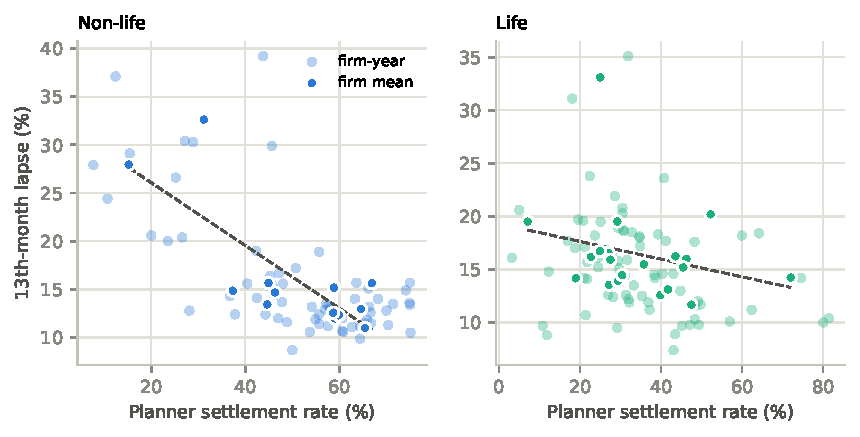
\includegraphics[width=0.95\linewidth]{fig/settle_lapse.pdf}
\caption{Planner settlement vs.\ 13th-month lapse, firm-years (light) and firm means (dark), with fit through firm means.}
\end{figure}
\begin{table}[H]\centering\small
\caption{Life insurers: lapse on planner settlement (FSS data only).}
\resizebox{\linewidth}{!}{\begin{tabular}{lcccccccc}
\toprule
 & \multicolumn{4}{c}{13th-month lapse$_t$} & \multicolumn{4}{c}{25th-month lapse$_t$} \\ \cmidrule(lr){2-5}\cmidrule(lr){6-9}
 & Pooled OLS & Random eff. & Firm FE & Two-way FE & Pooled OLS & Random eff. & Firm FE & Two-way FE \\
\midrule
Settlement$_t$ (\%) & $-0.092^{***}$ & $-0.120^{***}$ & $-0.135^{**}$ & $-0.049$ &  &  &  &  \\
 & $(0.035)$ & $(0.043)$ & $(0.059)$ & $(0.052)$ &  &  &  &  \\
Settlement$_{t-1}$ (\%) &  &  &  &  & $-0.046$ & $-0.047$ & $-0.214^{*}$ & $-0.074$ \\
 &  &  &  &  & $(0.046)$ & $(0.046)$ & $(0.122)$ & $(0.133)$ \\
\midrule
$N$ (firms) & 77 (20) & 77 (20) & 77 (20) & 77 (20) & 62 (19) & 62 (19) & 62 (19) & 62 (19) \\
$R^2$ (within for FE) & 0.09 & 0.29 & 0.13 & 0.02 & 0.01 & 0.01 & 0.08 & 0.02 \\
\bottomrule
\end{tabular}}
\end{table}
\noindent In life insurance higher settlement also goes with lower 13th-month lapse in pooled, RE and firm-FE
models (about $-0.12$), and the Hausman test does not reject RE ($p=0.56$). With year effects, however, the
coefficient falls to $-0.05$ ($p=0.35$). Life persistency moved sharply and in common across firms: the
industry 25th-month rate fell from 70.0\% (2022) to 60.7\% (2023) and recovered to 76.0\% (2025), largely through
bancassurance savings business \cite{fss}. Year effects absorb these swings, which leaves too little settlement-driven
variation to identify the effect. Life within-firm variation in lapse is also mostly bancassurance-driven, which the
exclusive-planner settlement rate does not measure.

%====================================================================
\section{Discussion}
%====================================================================
\paragraph{Interpretation.} The mis-selling--lapse correlation that is visible in any cross-section of Korean
insurers is a \emph{business-model} correlation. Telemarketing- and direct-led insurers typically sell simpler cover
remotely, with less needs analysis. They have both more quality-guarantee and complaint
cancellations and more early lapse. It does not follow that an insurer can cut its lapse rate by cutting its
measured mis-selling. The planner settlement rate, by contrast, carries within-firm information. When an
insurer's newly recruited planners stay, its business persists better a year later. This is consistent with
the ``orphan contract'' mechanism, where policies sold by planners who leave are less serviced and more likely
to lapse. It is also consistent with reverse causation through clawbacks: planners whose business lapses lose
commission and quit. Our lag structure (settlement in $t-1$ for 25th-month lapse) points in the same direction
but cannot rule this out.

\paragraph{Relevance to the commission reform.} The results support the reform's emphasis on sales-force
stability rather than on mis-selling metrics alone. These data cannot test settlement funds directly, but they show
that what matters for persistency is whether planners stay, not how many are recruited. A reform that shifts pay toward multi-year maintenance fees gives
planners a reason to stay and to keep their clients, which is exactly the channel through which settlement
relates to lapse here. Mis-selling statistics, as currently published, are too coarse and too dominated by
channel mix to serve as a within-firm early-warning indicator of lapse.

\paragraph{Limitations.}
\begin{itemize}
  \item \textbf{Small panel}: 13--14 non-life firms over 5 years; inference relies on few clusters (hence the bootstrap).
  \item \textbf{Measurement}: mis-selling is rounded to 1\,bp, which attenuates any within-firm slope. The
        settlement rate covers exclusive planners only, while persistency covers all channels, including GA and
        bancassurance business.
  \item \textbf{Mechanical overlap}: quality-guarantee and complaint cancellations are themselves early
        terminations. Their magnitude (bp) is negligible relative to lapse (pp), so this does not drive the results.
  \item \textbf{Causality}: TWFE removes fixed and common shocks but not time-varying firm strategy (e.g.\ a push into GA channels that changes both settlement and persistency).
  \item \textbf{Coverage}: life mis-selling data (Korea Life Insurance Association) were not part of the specified sources. Adding them would allow the full three-way analysis for life insurers.
\end{itemize}

%====================================================================
\section{Conclusion}
%====================================================================
Across Korean non-life insurers, mis-selling and lapse rise together, but only because some business models
generate both. Within an insurer over 2021--2025, changes in measured mis-selling do not predict changes in
lapse. The stability of the sales force does: a 10\,pp higher one-year planner settlement rate is associated
with about 1\,pp lower 13th-month lapse, robustly across estimators and samples. For supervisors this
suggests monitoring planner retention alongside, and perhaps ahead of, mis-selling ratios. For the 1200\% rule
and installment reforms it suggests the payoff will come through retention of planners as much as through
better sales conduct.

\appendix
\section{Reproducibility}\sloppy
\begin{itemize}
  \item \texttt{build\_panel.py}: parses the archived FSS/KNIA HTML in \texttt{data/} and writes \texttt{panel.csv}.
  \item \texttt{analysis.py}: correlation decomposition, panel regressions (\texttt{linearmodels}), wild cluster bootstrap, tables and figures.
  \item KNIA queries: POST to \texttt{/disclosure/item/04.do} and \texttt{07.do} with \texttt{\{04|07\}\_searchCode=YYYY\{F|L\}}.
        FSS queries: \texttt{list.do?menuNo=200414\&optn1=YYYYMM\&optn2=YYYYMM}.
\end{itemize}

\begin{thebibliography}{9}\small
\bibitem{fss} Financial Supervisory Service, \emph{2024 sales-channel efficiency of insurers and supervisory direction}, press release, 23 Apr 2025; and FSS insurance company disclosure, contract management (accessed 5 Oct 2026).
\bibitem{knia} General Insurance Association of Korea, consumer portal disclosures, items 04 (mis-selling) and 07 (claim denial), accessed 5 Oct 2026.
\end{thebibliography}
\end{document}
